\documentclass[12pt,conference]{IEEEtran}

% Store the title as a variable
\newcommand{\paperTitle}{Structural Quality \& Software Evolution}

% Preset Packages
\usepackage{cite} % Used to cite sources
\usepackage[hyphens]{url} % Used to prevent hypens in URLs
\usepackage{hyperref} % Used to make URLs clickable
\usepackage{graphicx} % Used to set the image path
\usepackage{xcolor} % Used to provide font color
\usepackage{csquotes} % Used to display quotes
\usepackage{setspace} % Used to provide line spacing

\def\BibTeX{{\rm B\kern-.05em{\sc i\kern-.025em b}\kern-.08em
    T\kern-.1667em\lower.7ex\hbox{E}\kern-.125emX}}

% Set the path to keep diagram images
\graphicspath{ {Images/} }

% Create a "todo" style (just red text)
\newcommand\todo[1]{\textcolor{red}{#1}}

% Create a "code" monospaced style
\newcommand{\code}[1]{\texttt{#1}}

% =============================================================================
% =  BEGINNING OF THE DOCUMENT
% =============================================================================
\begin{document}

% Include Page Numbers
\pagenumbering{arabic}
\pagestyle{plain}

% Set the title
\title{Initial Proposal: \paperTitle}

% Set the author information
\author{
\IEEEauthorblockN{Alison Major}
\IEEEauthorblockA{\textit{Department of Computer and Mathematical Sciences} \\
\textit{Lewis University}\\
Romeoville, Illinois, USA \\
AlisonMMajor@lewisu.edu}
}

% =============================================================================
% =  Paper Title & Author Information
% =============================================================================
\maketitle

% Set the document to be double spaced 
% http://kb.mit.edu/confluence/pages/viewpage.action?pageId=3907092
\doublespacing

When building software systems, we have several areas of concern: cost, delivery timeline, quality, etc. The cost and time-to-market are often the two problems given the highest priority in a project. However, engineers must consider the software quality to preserve the system's longevity. Despite its importance, the code and architecture quality can be challenging to understand and measure.

When we think about projects, we can assume that as time goes on and changes and additions occur within a system's source code, the complexity of that system will grow (``Fig.~\ref{figTimeAndComplexity}''). However, when we manage the code structure, we can keep the complexity in check, allowing systems to evolve. Developers can maintain this structure through simple steps like having readable code and more complex considerations, like how coupled and cohesive a system is.

\begin{figure}[ht]
    \centerline{
        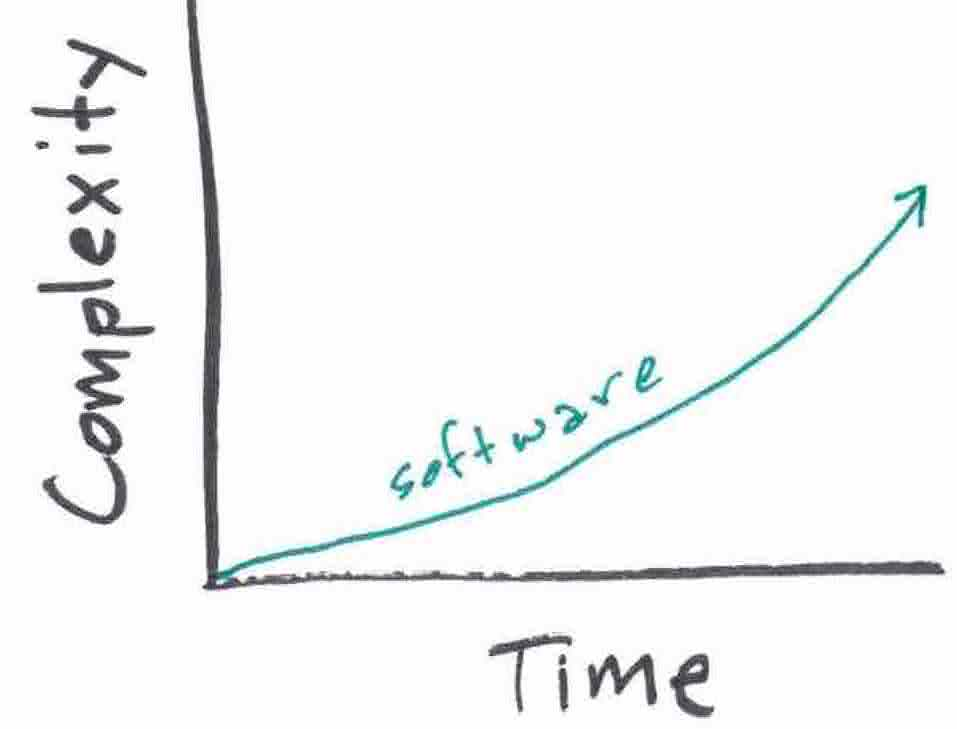
\includegraphics[width=0.7\columnwidth]{TimeAndComplexity}
    }
    \caption{Generally speaking, a software system will get more complex as it grows over time.}
    \label{figTimeAndComplexity}
\end{figure}

One way to understand the quality around a system is to discuss its ``maintainability,'' the ease of receiving new features or resolving bugs. For example, developers may find that adjusting one area to add a new feature requires touching several other code areas in tightly coupled systems. Some code measuring systems provide a Maintainability Index, a well-known quality measure. However, its effectiveness in quantifying software quality is debated \cite{vandeursen:2014}.

On the other hand, code smells are used extensively by practitioners to identify low-quality spots in the software system. These areas would need the teams' attention and are good candidates for refactoring.

Pylint is a static analysis tool that identifies several classes of code quality concerns, particularly relevant to our study, refactor violations, which report on various code smells. We can assume that there must be some correlation between Maintainability Index and the type and number of code smells in a software system, quantified by the Pylint refactor score.

This study explores such assumptions and systematically investigates any correlation between the Maintainability Index metric and the Pylint Refactor score. Furthermore, we perform analysis on specific refactor violations to reveal and shed light on the relative effectiveness of the different refactor violations and their relationship to Maintainability Index.

The structural quality of a software system will impact the software evolution. If the project has poor structural quality, the architecture will minimize its ability to evolve, and the software system will eventually ``die-off'' so to speak.

Why should we care about whether the code is maintainable? It is assumed that a large amount of the cost over the lifetime of a project is attributed to maintainability. Fred Brooks, in his book ``The Mythical Man-Month'' even claimed that over 90\% of the costs for a typical software system come up in the maintenance phase \cite{brooks:mythical}. Once the bulk of the system is off the ground and live worldwide, how well the team can improve the system with new features and fix bugs, even working on different parts in parallel, can be impacted by its maintainability. Any successful piece of software will inevitably need to be maintained.

We will look at many open-source Python systems using Pylint and attempt to correlate the data from the Pylint scores to the level of ease in adding new features to the system. This will determine if a system is more maintainable with better Pylint scores. 

In this study, we will be using Pylint and will be focused on the values of the Refactor score regarding a set of open-source Python systems. To understand the scores we will be working with; we must understand what Pylint itself is doing. 

Through the documentation of Pylint, we can understand how to use it and the scores it will provide \cite{pylint:main}. The Pylint score itself is calculated by the following equation \cite{pylint:score}:

\vspace{0.25cm}
\code{10.0-((float(5*e+w+r+c)/s)*10)}
\vspace{0.25cm}

Numbers closer to \code{10} reflect systems that have fewer errors, fewer warnings, and have overall better structure and consistency. In the above equation, we are using the following values \cite{pylint:docs}:

\vspace{0.25cm}
\begin{itemize}
    \item \textbf{statement} (\code{s}): the total number of statements analyzed
    \item \textbf{error} (\code{e}): the total number of errors, which are likely bugs in the code
    \item \textbf{warning} (\code{w}): the total number of warnings, which are python specific problems
    \item \textbf{refactor} (\code{r}): the total number of refactor warnings for bad code smells
    \item \textbf{convention} (\code{c}): the total number of convention warnings for programming standard violations
\end{itemize}
\vspace{0.25cm}

The Refactor score is of particular interest to us and considers many features that are meticulously outlined on the Pylint site \cite{pylint:refactor}. These types of warnings include several checks, such as when a boolean condition could be simplified, or a useless \code{return}, and so on. This score, in particular, will be part of our focus.

To calculate the Refactor score, Pylint will check the code for code smells based on the definitions for checks that have been documented. For every infraction, the score increases by one count. 

\vspace{0.25cm}
\begin{displayquote}
``In computer programming, a \textbf{code smell} is any characteristic in the source code of a program that possibly indicates a deeper problem.'' \cite{wiki:code-smells}
\end{displayquote}
\vspace{0.25cm}

We can use these Refactor scores to help us spot architecture smells. After all, code smells can point the way to deeper problems in our system. There are fundamental design principles that have been established that we should consider when creating software; code smells alert us to areas that have deviated from these principles. These smells are drivers for refactoring and when addressed, can help us maintain the integrity of our architecture rather than creating a patchwork construction.

Work done by Dr. Omari and Dr. Martinez involves collecting a sub-set of Python projects that we can use for further research. The bulk of the effort they have provided is determining which classifiers to use to pare down the public set of Python systems into a good collection for further analysis \cite{omari:2018}. The work that they have provided will be used to select appropriate Python systems for review by collecting meta-data on these code systems.

From their subset of repositories, we will then be able to collect current Pylint scores from each of our selected systems. This will give us a sampling of data that we can dig deeper into, comparing similar systems (similar size, similar number of contributors, etc.) and their evolution process by reviewing past commits rather than merely the current state of the system.

% =============================================================================
% =  Bibliography and Sources
% =============================================================================
\newpage

% Set line spacing for Bibliography
\setstretch{1.4}

\bibliographystyle{unsrt}
\bibliography{bibliography}

% =============================================================================
% =  END OF THE DOCUMENT
% =============================================================================
\end{document}
